\documentclass[a4paper,12pt]{article}
\usepackage[utf8]{inputenc}
\usepackage{amsmath}
\usepackage{amssymb}
\usepackage{bm} % to get bold epsilon
\usepackage{amssymb}
\usepackage{comment}
\usepackage{graphicx}
\usepackage{xcolor}
\usepackage[left=1.5cm, right=1.5cm, top=2cm, bottom=2cm]{geometry}
\title{\textbf{COM 5120 Communication Theory}}
\author{\textbf{Final Exam}}
\date{December 27, 2022\\
15:30 $\sim$ 17:20
}
\begin{document}
    \maketitle
    \textit{Note}: There are \textbf{6} problems with total 100 points within \textbf{2} pages, please write your answer with detail in the answer sheet.

    {\bf No credit without detail. Closed books. You may use scientific calculator.}

    \begin{enumerate}
     %%%%%%%%%%%%%%%%%%%%%%%%%%%%%%     
        \item (12\%)
            % 1. (Homework #2 - 3, 6.4)
            Let $X$ be a geometrically distributed random variable, i.e., $$P(X = k) = p(1-p)^{k - 1}, k = 1, 2, 3, ...$$
            (a) Find the entropy of $X$. \\ 
            (b) Given that $X > K$, where $K$ is a positive integer, what is the entropy of $X$? \\ 
    %%%%%%%%%%%%%%%%%%%%%%%%%%%%%%   
        \item (12\%)
            % 2. (Practice #3 - 2, 6.43)
            For the channel shown in Figure 1 and given that $P(A) = 1 - p, \ P(B) = P(C) = \frac{P}{2}$, \\
            find the channel capacity and the input distribution that achieves capacity. 
            \begin{figure}[h]
                \centering
                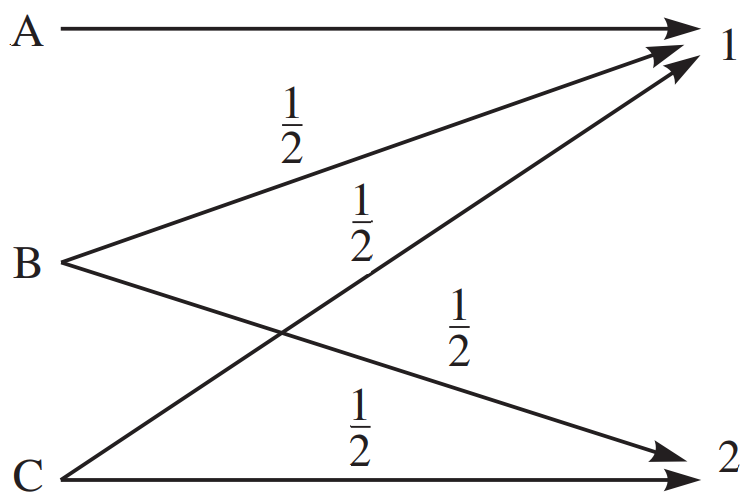
\includegraphics[scale=0.35]{Practice3-2-1.png}
                \caption{channel model}
                % \label{fig}
            \end{figure} \\ 
    %%%%%%%%%%%%%%%%%%%%%%%%%%%%%%
        \item (12\%)
            % 3. (Practice #3 - 2, 9.14)
            A voice-band telephone channel passes the frequencies in the band from $300$ to $3300$ Hz. It is desired to design a modem that transmits at a symbol rate of $2400$ symbols/s, with the objective of achieving $9600$ bits/s. \\
            Select an appropriate QAM signal constellation, carrier frequency, and the roll-off factor of a pulse with a raised cosine spectrum that utilizes the entire frequency band. \\
            Sketch the spectrum of the transmitted signal pulse and indicate the important frequencies. \\
    %%%%%%%%%%%%%%%%%%%%%%%%%%%%%%  
        \item (24\%) 
            % 4. (4.24)
            Three equiprobable messages $m_1$, $m_2$ and $m_3$ are to be transmitted over an AWGN channel with noise power spectral density $\frac{1}{2}N_0$. The messages are 
            \begin{align*}
                s_1(t) = \left\{
                \begin{aligned}
                    & 1 \;\;\;\; 0 \leq t \leq T \\ 
                    & 0 \;\;\;\; \text{otherwise}
                \end{aligned}
                \right.
                \;\;\;\;\;\;
                s_2(t) = -s_3(t) \left\{
                \begin{aligned}
                     &1  \;\;\;\; 0 \leq t \leq \frac{1}{2}T \\ 
                    -&1 \;\;\;\; \frac{1}{2}T < t \leq T \\
                     &0  \;\;\;\; \text{otherwise}
                \end{aligned}
                \right.
            \end{align*}
            (a) What is the dimensionality of the signal space? \\ 
            (b) Find an appropriate basis for the signal space. \\ 
            (c) Please Draw the signal constellation of the messages $m_1$, $m_2$, $m_3$ and the optimal decision regions $R_1$, $R_2$, $R_3$ for this problem. \\ 
            (d) Which of the three messages is most vulnerable to errors and why? In other words, which of $P(\text{error} \ | \ m_i \; \text{transmitted}), \ i = 1, 2, 3$, is largest? \\ 
    %%%%%%%%%%%%%%%%%%%%%%%%%%%%%%  
        \item (24\%)
            % 5. (6.28)
            Two discrete memoryless information sources X and Y each have an alphabet with six symbols, $\mathcal{X} = \mathcal{Y} = \{ 1, 2, 3, 4, 5, 6 \}$. 
            The probabilities of the letters for X are $\{ \frac{1}{2}$, $\frac{1}{4}$, $\frac{1}{8}$, $\frac{1}{16}$, $\frac{1}{32}$, $\frac{1}{32} \}$. The source Y has a uniform distribution. \\ 
            (a) Find the entropy of both X and Y. \\ 
            (b) Design Huffman codes for each source. Which Huffman code is more efficient? \\
            \textbf{(\textit{Hint}}: Efficiency of a Huffman code is defined as the ratio of the source entropy $H(X)$ to the average codeword length $\Bar{R}$.\textbf{)} \\ 
            (c) If Huffman codes were designed for the second extension of these sources (i.e., two letters at a time), for which source X or Y would you expect a performance improvement compared to the single-letter Huffman code and why? \\ 
    %%%%%%%%%%%%%%%%%%%%%%%%%%%%%%    
        \item (16\%)
            % 6. (9.42 + 9.41 ZF)
            The transmission of a signal pulse with a raised cosine spectrum through a channel results in the following \textbf{(noise-free)} sampled output from the demodulator: 
            \begin{align*}
                x_m = \left\{
                \begin{aligned}
                    -0.&5 \;\;\; m = -2 \\ 
                     0.&1 \;\;\; m = -1 \\ 
                       &1 \;\;\; m = 0 \\ 
                    -0.&2 \;\;\; m = 1 \\ 
                    0.0&5 \;\;\; m = 2 \\ 
                       &0 \;\;\; \text{otherwise} \\ 
                \end{aligned}
                \right.
            \end{align*}
            (a) Design a three-tap zero-forcing linear equalizer so that the output is 
            \begin{align*}
                q_m = \left\{
                \begin{aligned}
                    & 1 \;\;\; m = 0 \\ 
                    & 0 \;\;\; m = \pm 1 
                \end{aligned}
                \right.
            \end{align*}
            (b) Determine $q_m$ for $m = \pm 2, \pm 3$ by convolving the impulse response of the equalizer with the channel response. \\ 
    %%%%%%%%%%%%%%%%%%%%%%%%%%%%%%
    \end{enumerate}
    \rule{\textwidth}{0.4pt}
\end{document}
